\documentclass[
  % all of the below options are optional and can be left out
  % course name (default: 2IL50 Data Structures)
  course = {{16-811 Math Fundamentals for Robotics}},
  % quartile (default: 3)
  quartile = {{1}},
  % assignment number/name (default: 1)
  assignment = 5,
  % student name (default: Some One)
  name = {{Kangle Deng}},
  % student number, NOT S-number (default: 0123456)
  % studentnumber = {{0123456 ; 0314159}},
  % student email (default: s.one@student.tue.nl)
  email = {{kangled@andrew.cmu.edu}},
  % first exercise number (default: 1)
  firstexercise = 1
]{aga-homework}

\usepackage{subfigure}

\begin{document}

\exercise

Considering the small range $[x, x+dx]$, the curve $y(x)$ can be simplified as a line of length $\sqrt{1+y'^2(x)}dx$. The surface area of revolution is the side area of a frustum of core, whose radii are $y(x)$ and $y(x+dx)$. The area can be represented by:

\begin{equation*}
\begin{aligned}
      & \frac{1}{2}\pi (y(x)+y(x+dx)) \sqrt{1+y'^2(x)}dx \\ \approx & \frac{1}{2}\pi (y(x)+y(x)+y'(x)dx) \sqrt{1+y'^2(x)}dx
      \\ \approx & \pi y(x) \sqrt{1+y'^2(x)}dx
\end{aligned}
\end{equation*}

So we can formulate the problem as:

\begin{equation*}
    \min \limits_{y \in C^2} L(y) = \pi \int_{x_0}^{x_1} y \sqrt{1+y'^2}dx \qquad s.t. \quad y(x_0) = y_0,  y(x_1) = y_1.
\end{equation*}
Let $F(x,y,y') = y \sqrt{1+y'^2}$. From the Euler-Lagrange Equation, we have:

\begin{equation}
    F_y - \frac{d}{dx}F_{y'} = 0.
    \label{eq:hw5_ele}
\end{equation}

Note that:

\begin{equation*}
    \begin{aligned}
          \frac{d}{dx}(y'F_{y'}-F) & = y'\frac{d}{dx}F_{y'} + y''F_{y'
          } - F_x - y'F_y - y''F_{y'} \\
          & = -y'(F_y - \frac{d}{dx}F_{y'}) - F_x \qquad \qquad \text{(Plug in Eq. (\ref{eq:hw5_ele}))} \\
          & = -F_x = 0.
    \end{aligned}
\end{equation*}

So, 

\begin{equation*}
\begin{aligned}
  y'F_{y'}-F & = y'\frac{yy'}{\sqrt{1+y'^2}} - y \sqrt{1+y'^2} \\
  & = \frac{y}{\sqrt{1+y'^2}}[y'^2 - (1+y'^2)] \\
  & = \frac{-y}{\sqrt{1+y'^2}} = constant.
\end{aligned}

\end{equation*}

Let 

\begin{equation*}
    ky = \sqrt{1+y'^2},
\end{equation*}
where $k \ne 0$ is some constant.

So,

\begin{equation*}
    \begin{aligned}
     & ky = \sqrt{1+y'^2}, \\
     \Rightarrow \quad & k^2y^2 = 1 + y'^2, \\
     \Rightarrow \quad & k^2y^2 - 1 = y'^2, \\
     \Rightarrow \quad & \pm \sqrt{k^2y^2 - 1} = \frac{dy}{dx}, \\
     \Rightarrow \quad & \pm dx = \frac{dy}{\sqrt{k^2y^2 - 1}}, \\
     \Rightarrow \quad & \pm \int dx = \int \frac{dy}{\sqrt{k^2y^2 - 1}}, \\
    \end{aligned}
\end{equation*}

Since

\begin{equation*}
    \frac{d}{dy}[\ln(ky+\sqrt{k^2y^2-1})] = \frac{1}{ky+\sqrt{k^2y^2-1}}(k+\frac{k^2y}{\sqrt{k^2y^2-1}}) = \frac{k}{\sqrt{k^2y^2-1}},
\end{equation*}
we have: $\int \frac{dy}{\sqrt{k^2y^2 - 1}} = \frac{1}{k}\ln(ky+\sqrt{k^2y^2-1})$.

So,
\begin{equation*}
    \begin{aligned}
     & \pm (x + c) = \frac{1}{k}\ln(ky+\sqrt{k^2y^2-1}). \\
     \Rightarrow \quad & ky+\sqrt{k^2y^2-1} = e^{\pm k(x+c)}, \qquad\qquad \text{(a)}\\
     \Rightarrow \quad & \frac{1}{ky-\sqrt{k^2y^2-1}} = e^{\pm k(x+c)}, \\
     \Rightarrow \quad & ky-\sqrt{k^2y^2-1} = e^{\mp k(x+c)}, \qquad\qquad \text{(b)}\\
     \Rightarrow \quad & 2ky = e^{k(x+c)} + e^{-k(x+c)}, \qquad \text{(Adding (a) and (b))} \\
     \Rightarrow \quad & y = \frac{1}{2k}(e^{k(x+c)} + e^{-k(x+c)}) = \frac{1}{k}\cosh(k(x+c)).
    \end{aligned}
\end{equation*}

If the curve is not required to be $C^2$, it would be zero function except for the 2 endpoints. That is to say, $y = 0, \forall x \in (x_0,x_1)$ and $y(x_0) = y_0, y(x_1) = y_1$.

The endpoint conditions are used to determine the parameters $k$ and $c$ in the expression of $y = \frac{1}{k}\cosh(k(x+c))$.

\exercise

Use spherical $(u,v)$ coordinates, where $x=R\sin v \cos u, y = R\sin v\sin u, z = R \cos v$, with $R$ the radius of the sphere.

So,

\begin{equation*}
    \begin{aligned}
     dx & = R\cos v \cos u dv - R \sin v \sin u du, \\
     dy & = R\cos v \sin u dv + R \sin v \cos u du, \\
     dz & = -R\sin v dv.
    \end{aligned}
\end{equation*}

The differential arc-length can be represented by:

\begin{equation*}
    \begin{aligned}
     & \sqrt{dx^2+dy^2+dz^2} \\
     = & (R^2\cos^2v\cos^2udv^2 + R^2\sin^2v\sin^2udu^2 - 2R^2\sin v \cos v \sin u \ cos u du dv \\
     + & R^2\cos^2v\sin^2udv^2 + R^2\sin^2v\cos^2udu^2 + 2R^2\sin v \cos v \sin u \ cos u du dv \\
     + & R^2 \ sin^2 v dv^2)^\frac{1}{2}, \\
     = & \sqrt{R^2\cos^2vdv^2 + R^2\sin^2 v du^2 + R^2\sin^2vdv^2},\\
     = & R \sqrt{dv^2 + \sin^2vdu^2}, \\
     = & R \sqrt{v'^2 + \sin^2v} du.
    \end{aligned}
\end{equation*}

So the arc-length from $(u_0, v_0)$ to $(u_1, v_1)$ is:

\begin{equation*}
    L = R \int_{u_0}^{u_1} \sqrt{v'^2 + \sin^2v} du.
\end{equation*}

Let $F(u, v, v') = \sqrt{v'^2 + \sin^2v}$. Note that $F$ does not contain $u$. Similar to Problem 1, we have:
\begin{equation*}
    v'F_{v'} - F = a,
\end{equation*}
where $a$ is some constant.

So,

\begin{equation*}
\begin{aligned}
 &     \frac{v'^2}{\sqrt{v'^2+\sin^2v}} - \sqrt{v'^2 + \sin^2v} = a, \\
 \Rightarrow \quad & v'^2 - (v'^2 + \sin^2v) = a\sqrt{v'^2+\sin^2v}, \\
  \Rightarrow \quad & \sin^4v = a^2 (v'^2 + \sin^2v), \\
   \Rightarrow \quad & v'^2 = \frac{\sin^4 v - a^2\sin^2 v}{a^2}, \\
    \Rightarrow \quad & \frac{dv}{du} = \frac{\pm \sqrt{\sin^4 v - a^2\sin^2 v}}{a}, \\
\Rightarrow \quad & \frac{adv}{\sqrt{\sin^4 v - a^2\sin^2 v}} = \pm du, \\
\Rightarrow \quad & \int \frac{adv}{\sqrt{\sin^4 v - a^2\sin^2 v}} = \pm \int du, \\
\Rightarrow \quad & -\sin^{-1} (\frac{\cot v}{\sqrt{\frac{1}{a^2} - 1}}) = \pm (u + k), \\
\Rightarrow \quad & \sin(u+k)\tan v = \mp \frac{1}{\sqrt{\frac{1}{a^2} - 1}}.
\end{aligned}

\end{equation*}

Now we prove the equation $\sin(u+k)\tan v = c$ represents a great circle on the sphere. As shown in the Fig. \ref{fig:hw5_ex2}, suppose $\vec{OA}, \vec{OB}$ and $\vec{OC}$ denote the directions of x-axis, y-axis, and z-axis. We first study the great circle which is rotated from the equatorial plane around $OA$. The angle between this great circle plane and the equatorial plane is $\angle BOD = \theta$.

Suppose $P$ is a point on this great circle. $PE$ is the vertical line perpendicular to the equatorial plane. Also, we draw $PF \perp OA$, and connect $EF$. It is easy to show that $EF \perp OA$. Therefore, $\angle EFP$ is also the angle $\theta$ between the great circle plane and the equatorial plane.

From the perspective of spherical $(u,v)$ coordinates, $\angle COP = v$ and $\angle AOE = u$. Then we have $PE = R \cos v$ and $EF = R \sin v \sin u$. So $\tan \theta = \frac{PE}{EF} = \frac{\cos v}{\sin v \sin u} = \frac{1}{\tan v \sin u}$.

Therefore, all the points on this great circle satisfies that $\tan v \sin u$ remains a constant. Furthermore, any great circle on the sphere can rotate to such a circle we mentioned above around $OC$, which means $\tan v \sin (u+k)$ remains a constant.

In conclusion, the equation  $\sin(u+k)\tan v = c$ we get from the Calculus of Variations represents some great circle on the sphere.

\begin{figure}
    \centering
    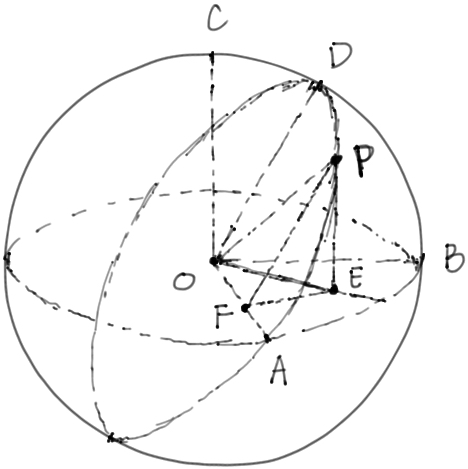
\includegraphics[width=.4\textwidth]{math/fig/hw5/hw5_ex2.jpeg}
    \caption{Illustration of Ex. 2}
    \label{fig:hw5_ex2}
\end{figure}

\exercise

From the lecture, we know such equation holds at $(x_1, y_1)$:

\begin{equation*}
    F_{y'} - \frac{g_yF}{g_x+y'g_y} = 0.
\end{equation*}

Then we plug in $F$ and $F_y'$ by:

\begin{equation*}
    \begin{aligned}
     F  & = \frac{\sqrt{1+y'^2}}{\sqrt{y_0-y}}, \\
     F_{y'} & = \frac{y'}{\sqrt{(y_0-y)(1+y'^2)}}.
    \end{aligned}
\end{equation*}

So,

\begin{equation*}
    \begin{aligned}
     & \frac{y'}{\sqrt{(y_0-y)(1+y'^2)}} = \frac{g_y}{g_x+y'g_y} \cdot \frac{\sqrt{1+y'^2}}{\sqrt{y_0-y}}, \\
     \Rightarrow \qquad & y' = \frac{g_y}{g_x+y'g_y} \cdot (1+y'^2), \\
     \Rightarrow \qquad & y'g_x + y'^2g_y = g_y + y'^2g_y, \\
     \Rightarrow \qquad & y'g_x = g_y, \\
     \Rightarrow \qquad & y'= \frac{g_y}{g_x}.
    \end{aligned}
\end{equation*}

The direction of the curve $y(x)$ at $(x_1, y_1)$ can be represented by the vector: $(1, y'(x_1))^T$. Since we have $y'= \frac{g_y}{g_x}$ at $(x_1, y_1)$, $(1, y'(x_1))^T$ is parallel to the gradient of $g(x,y)$: $(g_x, g_y)^T$. Therefore, $y(x)$ intersects the iso-contour $g(x,y)=0$ orthogonally.

\exercise
\subexercise

Let $v_1$ denote the velocity of $m_1$, $v_{2A}$ denote the velocity of the upper $m_2$, and $v_{2B}$ denote the velocity of the lower $m_2$. 

For $v_1$, we have:

\begin{equation*}
    v_1 = l_1 \Dot{\theta_1}.
\end{equation*}

So,
\begin{equation*}
    v_1^2 = l_1^2 \Dot{\theta_1}^2.
\end{equation*}

To obtain $v_{2A}$ and $v_{2B}$, we consider the coordinates $(x_A, y_A)$ and $(x_B, y_B)$ of the 2 $m_2$:

\begin{equation*}
    \begin{aligned}
     x_A & = l_1\cos\theta_1 + l_2\cos(\theta_1+\theta_2), \\
     y_A & = l_1\sin\theta_1 + l_2\sin(\theta_1+\theta_2), \\
     x_B & = l_1\cos\theta_1 - l_2\cos(\theta_1+\theta_2), \\
     y_A & = l_1\sin\theta_1 - l_2\sin(\theta_1+\theta_2). \\
    \end{aligned}
\end{equation*}

Taking the derivative of the coordinates, we have:

\begin{equation*}
    \begin{aligned}
     \Dot{x_A} & = -l_1\sin\theta_1\Dot{\theta_1} - l_2\sin(\theta_1+\theta_2)(\Dot{\theta_1}+\Dot{\theta_2}), \\
     \Dot{y_A} & = l_1\cos\theta_1\Dot{\theta_1} + l_2\cos(\theta_1+\theta_2)(\Dot{\theta_1}+\Dot{\theta_2}), \\
     \Dot{x_B} & = -l_1\sin\theta_1\Dot{\theta_1} + l_2\sin(\theta_1+\theta_2)(\Dot{\theta_1}+\Dot{\theta_2}), \\
     \Dot{y_B} & = l_1\cos\theta_1\Dot{\theta_1} - l_2\cos(\theta_1+\theta_2)(\Dot{\theta_1}+\Dot{\theta_2}), \\
    \end{aligned}
\end{equation*}

So,

\begin{equation*}
    \begin{aligned}
     v_{2A}^2 = \Dot{x_A}^2 + \Dot{y_A}^2 = l_1^2\Dot{\theta_1}^2 + l_2^2(\Dot{\theta_1}+\Dot{\theta_2})^2 + 2l_1l_2\cos\theta_2\Dot{\theta_1}(\Dot{\theta_1}+\Dot{\theta_2}), \\
     v_{2B}^2 = \Dot{x_B}^2 + \Dot{y_B}^2 = l_1^2\Dot{\theta_1}^2 + l_2^2(\Dot{\theta_1}+\Dot{\theta_2})^2 - 2l_1l_2\cos\theta_2\Dot{\theta_1}(\Dot{\theta_1}+\Dot{\theta_2}). \\
    \end{aligned}
\end{equation*}

Since there is no gravity, we have:

\begin{equation*}
\begin{aligned}
    L & = \frac{1}{2}m_1v_1^2 + \frac{1}{2}m_2v_{2A}^2 + \frac{1}{2}m_2v_{2B}^2 \\
    & = \frac{1}{2}(m_1 + 2m_2)l_1^2\Dot{\theta_1}^2 + m_2l_2^2(\Dot{\theta_1}+\Dot{\theta_2})^2.
\end{aligned}
\end{equation*}

So,
\begin{equation*}
    \begin{aligned}
        \frac{\partial L}{\partial \theta_1} & = 0,\\
        \frac{\partial L}{\partial \theta_2} & = 0, \\
        \frac{\partial L}{\partial \Dot{\theta_1}} & = (m_1 + 2m_2)l_1^2\Dot{\theta_1} + 2m_2l_2^2(\Dot{\theta_1}+\Dot{\theta_2}), \\
        \frac{\partial L}{\partial \Dot{\theta_2}} & = 2m_2l_2^2(\Dot{\theta_1}+\Dot{\theta_2}).
    \end{aligned}
\end{equation*}

Therefore,
\begin{equation*}
    \begin{aligned}
        \tau_1 & = \frac{d}{dt}\frac{\partial L}{\partial \Dot{\theta_1}} - \frac{\partial L}{\partial \theta_1} = [(m_1+2m_2)l_1^2+2m_2l_2^2]\Ddot{\theta_1} + 2m_2l_2^2\Ddot{\theta_2}, \\
        \tau_2 & = \frac{d}{dt}\frac{\partial L}{\partial \Dot{\theta_2}} - \frac{\partial L}{\partial \theta_2} = 2m_2l_2^2\Ddot{\theta_1} + 2m_2l_2^2\Ddot{\theta_2}.
    \end{aligned}
\end{equation*}

\subexercise

When $\Ddot{\theta_2} = 0$,
\begin{equation*}
    \tau_1 = [(m_1+2m_2)l_1^2+2m_2l_2^2]\Ddot{\theta_1} = m_1l_1^2\Ddot{\theta_1} + 2m_2(l_1^2+l_2^2)\Ddot{\theta_1}.
\end{equation*}

In this formulation, $m_1l_1^2\Ddot{\theta_1}$ is the torque that keeps $m_1$ moving with an angle acceleration of $\Ddot{\theta_1}$.

On the other hand, $2m_2(l_1^2+l_2^2)\Ddot{\theta_1}$ also keeps the 2 $m_2$ moving with an angle acceleration of $\Ddot{\theta_1}$. To understand this, we consider the distance of the 2 $m_2$ from the origin. For the upper $m_2$, the square of distance is $l_1^2+l_2^2+2l_1l_2\cos \theta_2$ (derived from Law of Cosines). Similarly for the lower $m_2$, the square of distance is $l_1^2+l_2^2-2l_1l_2\cos \theta_2$. Therefore, the sum of these 2 squares is $2(l_1^2+l_2^2)$, which is consistent with the torque.

\end{document}